\documentclass{beamer}

\hypersetup{pdfstartview={Fit}}

\begin{document}

	\title[Crisis] % (optional, only for long titles)
	{Mesh to Voxel Transformations for Optimised Physics-Based Interactions}
	\subtitle{}
	\author[Lefley, Ponjou-Tasse] % (optional, for multiple authors)
	{T.~Lefley \and F.~Ponjou-Tasse}

	\date[2015] % (optional)
	{Project Presentation, 2015}
	\subject{Computer Science}

	\frame{\titlepage}

	\begin{frame}
	\frametitle{Motivation}
		\begin{columns}[T] % contents are top vertically aligned
			\begin{column}[T]{5cm} % each column can also be its own environment
				\begin{figure}
					\centerline{\includegraphics[scale=0.2]{diagram.pdf}}
					\caption{A simple collision and its volumetric resolution.}
				\end{figure}
			\end{column}
			\begin{column}[T]{5cm} % alternative top-align that's better for graphics
				\begin{itemize}
				\item{Meshes only store surface information}
				\item{Reasoning on interior difficult}
				\item{Most destruction algorithms limited}
					\begin{itemize}
							\item{Only work on convex shapes}
							\item{Or have to split concave shapes first}
					\end{itemize}
				\end{itemize}
				\begin{itemize}
				\item{By precomputing volume data we have an O(1) check for inside/outside a shape}
				\end{itemize}
			\end{column}
		\end{columns}	
	\end{frame}
	\begin{frame}
	\frametitle{Voxelisation}
		\begin{columns}[T] % contents are top vertically aligned
			\begin{column}[T]{5cm} % each column can also be its own environment
				\begin{figure}
					\centerline{\includegraphics[scale=0.4]{Voxelise.png}}
					\caption{Voxelisation of the `Stanford Bunny' model, composed of 69,666 triangles.}
				\end{figure}
			\end{column}
			\begin{column}[T]{5cm} % alternative top-align that's better for graphics
				\begin{itemize}
				\item{HLSL GPU algorithm}
				\item{Based on GPU Pro 3 implementation of Schwarz and Seidel's method}
				\item{Achieves solid voxelisation of convex and concave bodies}
				\end{itemize}
			\end{column}
		\end{columns}
	\end{frame}
	\begin{frame}
	\frametitle{Destruction}
		\begin{columns}[T] % contents are top vertically aligned
			\begin{column}[T]{5cm} % each column can also be its own environment
				\begin{figure}
					\centerline{\includegraphics[scale=0.5]{Voronoi.png}}
					\caption{Labelling of voxels to their correct fragments.}
				\end{figure}
			\end{column}
			\begin{column}[T]{5cm} % alternative top-align that's better for graphics
				\begin{itemize}
				\item{Process collision information}
					\begin{itemize}
						\item{Find collision point} 
						\item{Calculate force}
						\item{Generate fragment points}
					\end{itemize}
				\item{Construct 3D voronoi diagram}
					\begin{itemize}
						\item{Label each voxel by nearest point}
						\item{Within radius}
					\end{itemize}
				\item{Find islands}
					\begin{itemize}
						\item{Flood fill}
					\end{itemize}
				\end{itemize}
			\end{column}
		\end{columns}
	\end{frame}
	\begin{frame}
	\frametitle{Rebuilding the Mesh}
	\framesubtitle{Different Approaches}
		\begin{columns}[T] % contents are top vertically aligned
			\begin{column}[T]{5cm} % each column can also be its own environment
				\begin{figure}
					\centerline{\includegraphics[scale=0.4]{Marching.png}}
					\caption{Fractured Stanford Bunny remeshed using the Marching Tetrahedrons algorithm.}
				\end{figure}
			\end{column}
			\begin{column}[T]{5cm} % alternative top-align that's better for graphics
				\begin{itemize}
				\item{Marching Tetrahedra}
					\begin{itemize}
						\item{Original mesh not preserved}
						\item{Detail loss}
					\end{itemize}
				\end{itemize}
			\end{column}
		\end{columns}
	\end{frame}
	\begin{frame}
	\frametitle{Rebuilding the Mesh}
	\framesubtitle{Different Approaches}
		\begin{columns}[T] % contents are top vertically aligned
			\begin{column}[T]{5cm} % each column can also be its own environment
				\begin{figure}
					\centerline{\includegraphics[scale=0.5]{Porcelain.png}}
					\caption{Fractured Stanford Bunny mesh partitioned using nearest neighbour.}
				\end{figure}
			\end{column}
			\begin{column}[T]{5cm} % alternative top-align that's better for graphics
				\begin{itemize}
				\item{Marching Tetrahedra}
					\begin{itemize}
						\item{Original mesh not preserved}
						\item{Detail loss}
					\end{itemize}
				\item{Nearest Neighbour}
					\begin{itemize}
						\item{Find only fragment edge voxels}
						\item{Add them to KDTree}
						\item{For all vertices, map to nearest voxel}
					\end{itemize}
				\end{itemize}
			\end{column}
		\end{columns}
	\end{frame}
	\begin{frame}
	\frametitle{Rebuilding the Mesh}
	\framesubtitle{Different Approaches}
		\begin{columns}[T] % contents are top vertically aligned
			\begin{column}[T]{5cm} % each column can also be its own environment
				\begin{figure}
					\centerline{\includegraphics[scale=0.5]{Porcelain2.png}}
					\caption{Fractured hollow Stanford Bunny.}
				\end{figure}
			\end{column}
			\begin{column}[T]{5cm} % alternative top-align that's better for graphics
				\begin{itemize}
				\item{Marching Tetrahedra}
					\begin{itemize}
						\item{Original mesh not preserved}
						\item{Detail loss}
					\end{itemize}
				\item{Nearest Neighbour}
					\begin{itemize}
						\item{Find only fragment edge voxels}
						\item{Add them to KDTree}
						\item{For all vertices, map to nearest voxel}
					\end{itemize}
				\item{Meshing interior...}
				\end{itemize}
			\end{column}
		\end{columns}
	\end{frame}
	\begin{frame}
	\frametitle{The Next Steps}	
		\begin{itemize}
		\item{Finish interior meshing algorithm}
		\item{Optimise for speed}
			\begin{itemize}
				\item{Multithreading}
				\item{Remove unnecessary complexity}
			\end{itemize}
		\item{Post destruction calculations}
			\begin{itemize}
				\item{Fragment mass}
			\end{itemize}
		\item{Evaluation}
			\begin{itemize}
				\item{Framerate}
				\item{Memory usage}
				\item{Physical accuracy}
			\end{itemize}
		\item{Write-up}
		\end{itemize}
	\end{frame}

\end{document}